\documentclass[12pt]{article}
\usepackage{tikz}
\usepackage{algorithmicx}
%\usepackage[pagebackref=true,colorlinks,linkcolor=blue,citecolor=magenta]{hyperref}
\usepackage{graphicx} 
\usepackage{fancybox}
\usepackage{setspace}  
\usepackage[colorlinks,linkcolor=blue,citecolor=magenta]{hyperref}
\usepackage{enumerate} 
\usepackage{amsthm,amssymb,amsmath}
\usepackage{indentfirst}

\begin{document}

\title{Draft}
\date{}
\maketitle
\section{Join Tree}
Throughout these sections, for the sake of simplicity, we are dealing only with Boolean Conjunctive Query (BCQ) and we call them query. These result can be extended to other queries. 
Let fix a given query  as $Q$. Suppose for $Q$  we have its join tree $JT_{Q}<V>$ which $V, |V|=n$ represents the set of its nodes (i.e. Figure \ref{fig1}). 
This join tree has several nice properties. The most important property of join trees is that we can compute their results in linear time ???.
The other important property of join trees is \emph{connectedness property}. By the connectedness we mean that if we select a variable which occurs in the given query, ???. 

%\usetikzlibrary{positioning,shadows,arrows}
\begin{figure}[htbp]
\begin{center}
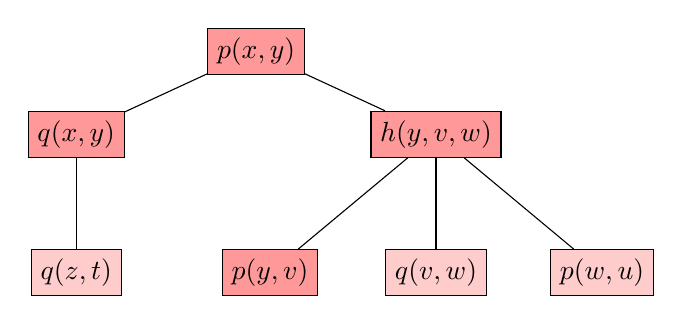
\begin{tikzpicture}%[level/.style={sibling distance=40mm,level distance=15mm}]
[
    %
    level 1/.style={rectangle, draw,scale=1.0, fill=red,
    level distance=30pt, sibling distance=130pt},
    level 2/.style={rectangle, draw, scale=1.0,
    level distance=50pt, sibling distance=60pt}]
    \tikzstyle{every node}=[rectangle,draw,fill=red!20]
    \node[fill=red!40] {$p(x,y)$}
        child { 
            node [fill=red!40] {$q(x,y)$}
            child { node {$q(z,t)$}} 
        }
        child { 
        		node[fill=red!40]  {$h(y,v,w)$}
		child{ node[fill=red!40]{$p(y,v)$}}
		child{node{$q(v,w)$}}
		child{node{$p(w,u)$}}
		}
    ;
\end{tikzpicture}
\end{center}
\caption{A sample join tree of a query}
\label{fig1}
\end{figure}
\subsection{Number of different nodes is polynomial}
Let fix $k$ as the tree width of given $JT_{Q}$. Here we consider the case when $k$ is constant (we have an upper bound for that).
When we apply the $\Delta$-operator to a join tree its nodes change also the structure. Here we prove that the number of all nodes in all different trees that emerge from all different sequence of applying the $\Delta$-operator is polynomial in term of $n$ for a fixed $k$.\\

The nodes of $JT_{Q}$ are all in form of $R_{i_{1}}\bowtie\cdots\bowtie R_{i_{m}}$ which $m\leq k$, $m$ relations join together. Lets fix one particular node as $l$ with $m$ relations and the set of its indices is $I$. If we apply $\Delta_{\pm R_{i_{p}}}$ when $i_{p}\not\in I$ this node is $\emptyset$. For the other case we will have node $R_{i_{1}}\bowtie\cdots R_{i_{p-1}}\bowtie R_{i_{p+1}}\cdots R_{i_{m}}$, in the other words relation $R_{i_{p}}$ was deleted from the join operation. Thus, for counting the number of all nodes in all $JT_{Q}$ for all sequences of applying $\Delta$-operator, we should count all nodes which contain $1,2,\cdots,k$ different relations. This number is 
$\sum_{i=1}^{k}{\binom{n}{i}}<(n+1)^{k}$ which is polynomial for a fixed $k$. \\

\subsection{Cost of Evaluation}
According to the last section the number of nodes in all delta trees is polynomial for a fixed $k$. Now we want to prove that the structures of all these trees are polynomial for a fixed $k$. \\

\begin{figure}[htbp]
\begin{center}
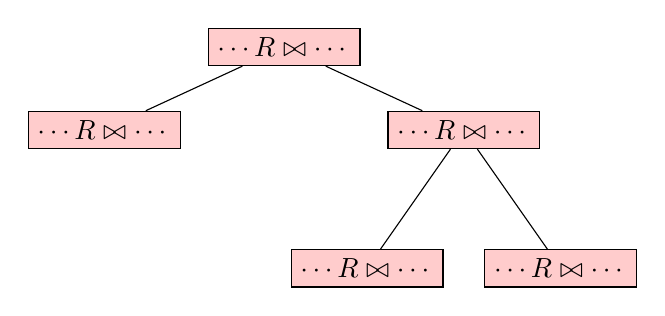
\begin{tikzpicture}%[level/.style={sibling distance=40mm,level distance=15mm}]
[
    %
    level 1/.style={rectangle, draw,scale=1.0, fill=red,
    level distance=30pt, sibling distance=130pt},
    level 2/.style={rectangle, draw, scale=1.0,
    level distance=50pt, sibling distance=70pt}]
    \tikzstyle{every node}=[rectangle,draw,fill=red!20]
    \node {$\cdots R\bowtie \cdots$}
        child { 
            node {$\cdots R\bowtie \cdots$}
        }
        child { 
        		node {$\cdots R\bowtie \cdots$}
		child{
       		node {$\cdots R\bowtie \cdots$}
		}
		child{
       		node {$\cdots R\bowtie \cdots$}
		}		
	}
    ;
\end{tikzpicture}
\end{center}
\caption{}
\label{fig2}
\end{figure}

When $\Delta_{R}$-operator applies to a join tree it doesn't change the nodes that do not contain $R$ relation. Thus, without loss of generality we can assume that $R$ has appeared in all nodes, since we have connectedness property. 

When we apply $\Delta_{R}$-operator the such a tree, each node splits into 3 different nodes($\Delta(R\bowtie S)=\Delta(R)\bowtie S+R\bowtie\Delta(S)+\Delta(R)\bowtie\Delta(S)$). If we consider each $+,\bowtie$ as one operation, evaluation of $\Delta(R\bowtie S)$ needs at most 5 operations. Thus, the cost of evaluation of all $\Delta$ trees is $O(n)*(\text{Cost of join operator})$.


\subsection{Hypertree Decomposition}
Gottlob et al. have shown that for each Hypertree there exists a join tree with the same tree structure(Lemma 4.6). Thus, we have these results for hypertrees too.
\end{document}
